\chapter{Marco teórico}

    En el área de visión computacional la estimación de la pose de una cabeza es el proceso de inferir la orientación y la posición de una cabeza humana a partir de las imágenes [Murphy et al, 2009]. El estimador debe ser robusto a distorsiones causadas por la cámara, a las expresiones faciales, al cabello, al vello facial y a objetos que ocluyan la cabeza como por ejemplo unos lentes o sombreros.\\
    Existen algunos aspectos que se deben tomar en cuenta al realizar investigación en de este tema: se necesita previamente localizar la cabeza de las personas; la cabeza humana puede ser modelada como un objeto rígido sin tomar en cuenta el resto del cuerpo humano; la estimación de la pose de la  cabeza se hace con respecto a un marco de referencia centrado en la cámara y de manera más general a un sistema global de coordenadas; para estimar la mirada de las personas con precisión en cualquier configuración un sistema seguidor de ojos debe ser complementado con el sistema de estimación de la  pose de la cabeza. [Wang et al, 2009].\\
    Actualmente se han realizado  una gran diversidad de métodos que se pueden emplear para solucionar el problema de la estimación de la pose de la cabeza, razón por la cual motivó a Murphy-Chutorian y Manubhai a desarrollar una taxonomía sobre los enfoques más importantes, en ella se presenta la clasificación de los métodos tomando como principal parámetro de clasificación el enfoque fundamental sobre el cual subyace la implementación del método. Las clasificaciones son:
    \begin{itemize}
    	\item \textit{Métodos de apariencias de plantillas}.- Este método utiliza métricas de comparación basadas en imágenes para hacer correspondencias de la pose de una cabeza con un conjunto de ejemplos (plantillas) con las poses etiquetadas, hace la correspondencia con las más similares de las plantillas. El método no requiere entrenamiento con ejemplos negativos, solo requiere los ejemplos etiquetados.\\
    	Desventajas:
    	\begin{enumerate}[label=(\alph*)]
    		\item Solo estiman posiciones discretas
    		\item Se requiere saber dónde se localiza el rostro
    		\item Ineficiente con muchos ejemplos
    		\item Ineficiente con imágenes de la misma persona del entrenamiento y durante la prueba
    	\end{enumerate}
%    Como posible solución a la ineficiencia en la detección y después estimación de pose se propone: SVM
%    Posible solución a los errores de estimación: filtro Laplacian-of-Gaussian	
\item \textit{Métodos detectores en forma de arreglo}.- Se entrenan múltiples detectores de rostro con diferentes poses discretas, la diferencia con el método anterior es que la imagen de entrada es evaluada con un detector entrenado con bastantes imágenes y un algoritmo supervisado.
\\Ventajas:
\begin{enumerate}[label=(\alph*)]
	\item La detección y localización no son etapas diferentes
	\item Son buenos con imágenes con alta y baja resolución
\end{enumerate}
Desventajas:
\begin{enumerate}[label=(\alph*)]
	\item Se requieren bastantes imágenes de entrenamiento
	\item Es difícil implementar el arreglo con un número de detectores  extenso en un sistema en tiempo real
	\item Podrían darse ambigüedades en la clasificación (múltiples clasificaciones positivas).
\end{enumerate}

\item \textit{Métodos de regresión no lineal}.- Estiman la pose mediante el aprendizaje de una función no lineal de mapeo desde un espacio de imágenes a una o más direcciones de pose. Con un conjunto de entrenamiento se puede construir un modelo que estime de forma discreta o continua una pose.
\\Desventajas:
\begin{enumerate}[label=(\alph*)]
	\item No es claro cómo se utilizará la herramienta específica de la regresión
	\item La estimación realizada es tosca (coarse) en las ubicaciones discretas
	\item Son propensas al error
\end{enumerate}

Las ventajas de utilizar este método con redes neuronales son:
\begin{enumerate}[label=(\alph*)]
	\item Bastante rápidos
	\item Solo requieren imágenes etiquetadas para entrenamiento
	\item Arrojan los resultados más exactos en la práctica.
\end{enumerate}

\item \textit{Métodos de variedad-embebida o manifold}.- Este método busca manifolds de baja dimensión que modelen la variación continua en la pose de la cabeza. Nuevas imágenes pueden ser incrustadas en estos manifolds y después utilizarlos para la estimación con técnicas como la regresión en el espacio embebido. Cualquier algoritmo de reducción de dimensionalidad puede ser considerado como un intento de un manifold embebido, pero la dificultad yace en crear un algoritmo que exitosamente recupere la pose de la cabeza mientras ignora otras fuentes de variación en la imagen.
\\Desventajas:
\begin{enumerate}[label=(\alph*)]
	\item Al igual que con los detectores en forma de arreglo la estimación de la pose es tosca ya que la estimación se deriva de un conjunto discreto de mediciones.
	\item La heterogeneidad en los datos de entrenamiento que es común en muchos escenarios de entrenamiento en el mundo real, representan un problema. Para contrarrestar lo anterior es necesario entrenar un manifold con múltiples personas, pero a menudo es imposible obtener un muestreo regular de poses de cada individuo.
\end{enumerate}
Ventajas:
\begin{enumerate}[label=(\alph*)]
	\item Todas las técnicas de variedad-embebida que utilicen un enfoque lineal tienen la gran ventaja de que la reducción de las dimensiones del modelo de la pose se puede lograr con unas simples multiplicaciones de matrices lo cual es bastante veloz en comparación con otros métodos.
\end{enumerate}

\item \textit{Modelos flexibles}.- Los modelos flexibles toman un enfoque diferente al de los métodos previos. En esta técnica un modelo no rígido es adaptado a la imagen de tal forma que se ajusta a la estructura facial de cada individuo, este método requiere datos de entrenamiento con las características del rostro anotados (comentados), permite hacer comparaciones a nivel características en lugar de a nivel global de apariencias. Básicamente los modelos son plantillas basadas en grafos deformables de puntos característicos locales del rostro como las esquinas de los ojos, nariz, boca, etc. Para entrenar este sistema las locaciones de las características de los rostros son etiquetadas a mano en cada imagen de entrenamiento. Estas características pueden ser extraídas de vistas de múltiples personas y extra invarianza puede ser lograda almacenando muchos descriptores en cada nodo, a esto se le conoce como Elastic Bunch Graph, además, tiene la capacidad de representar objetos no rigidos o deformables. \\
El proceso de pareo (matching) se realiza con el algoritmo Elastic Graph Matching, con éste se compara un conjunto de grafos con la imagen nueva, para ello se coloca el grafo sobre la imagen y se calculan las distancias mínimas de la característica en cada locación del nodo del grafo. \\
Para la estimación de la pose un conjunto de grafos es creado para cada pose discreta y es comparada con una nueva vista de la cabeza. El conjunto de grafos con mayor similitud asigna una pose discreta a la cabeza.
\\Desventajas:
\begin{enumerate}[label=(\alph*)]
	\item La estimación de la pose es discreta, requiriendo muchos conjuntos de grafos y comparar los conjuntos con muchas deformaciones resulta costoso computacionalmente.
	\item No es eficiente estar localizando todas las características de la cara en cada frame.
	\item Podría no estimar exitosamente la pose del rostro en imágenes de baja resolución y con el rostro lejos de la cámara.
\end{enumerate}

Ventajas:
\begin{enumerate}[label=(\alph*)]
	\item  Los modelos de apariencia activa (AAM) los cuales evolucionaron de modelos flexibles tienen buena invarianza al error de localización de la cabeza ya que ellos se adaptan a las imágenes y encuentran la posición exacta de las características de la cara.
\end{enumerate}

\textit{Métodos geométricos}.- Utilizan la forma de la cabeza y la configuración de las características locales para estimar la pose. El movimiento de yaw puede ser calculada con la distancia entre los ojos, roll con el ángulo que se forma con la línea de los ojos y el horizonte y pitch con la distancia de la punta de la nariz y la línea de los ojos.
\\Desventajas:
\begin{enumerate}[label=(\alph*)]
	\item Se necesita que el rostro se encuentre cerca de la cámara para ver todas las líneas del rostro.
	\item Es difícil es encontrar las características con alta precisión y exactitud.
	\item Son métodos sensibles a las oclusiones en la cara.
\end{enumerate}
Ventajas:
\begin{enumerate}[label=(\alph*)]
	\item Los métodos geométricos son rápidos y simples, con unas pocas características del rostro se puede obtener un decente estimador de la pose de la cabeza.
	\item Con muy simples características geométricas se puede estimar la pose de la cabeza, por ejemplo: el movimiento de yaw puede ser obtenido creando el triángulo entre los ojos y la boca y buscando el triángulo la desviación a partir de un triángulo isosceles puro.
\end{enumerate}


%Para la estimación de la pose el manifold debe ser modelado y una técnica de incrustación (embedding) es requerida para proyectar una nueva muestra dentro del manifold. Esta incrustación puede ser usado para la estimación de la pose con técnicas tales como la regresión en el espacio embebido

\end{itemize}
\subsection{Métodos para la recolección del ground truth}
Para evaluar y comparar los sistemas de estimación de pose se necesita de un método preciso para medir los datos de campo (ground truth) en un conjunto de datos evaluativos. Generalmente el "ground truth" es esencial para el entrenamiento en cualquier método de estimación de la pose. La siguiente lista describe los métodos más comunes para capturar estos datos de campo, en orden del menos preciso (burdo) al más preciso:
\begin{itemize}
	\item Sugerencia direccional.- Se les indica a las personas que miren hacia objetos en la habitación en la que se encuentran y se capturan las posiciones de la cabeza, no es muy preciso este método ya que entre otras cosas se asume que una persona tiene la habilidad de dirigir su cabeza con exactitud hacia los objetos.
	\item Sugerencia direccional con apuntador láser.- Igual al anterior pero con un láser, presenta los mismos problemas que el método anterior y las personas tienden a mover sus cabezas durante la captura de datos.
	\item Anotación manual.- Otras personas anotan la posición de la pose.
	\item Arreglo de cámaras.- Se capturan imágenes con múltiples cámaras a la misma persona con diferentes ángulos.
	\item Sensores magnéticos.- Los sensores se colocan en la cabeza de las personas y se obtienen las medidas del sensor. Entre las desventajas es que son sensibles al ruido y presencia de metales.
	\item Sensores inerciales.- Utilizan acelerómetros y giroscopios y se reduce el ruido con un filtro de kalman. No miden posición solo orientación en tres DOF.
	\item Sistemas ópticos de captura de movimiento.- Son robustos y muy costosos, son usados en captura profesional del movimiento articulado del cuerpo.	
\end{itemize}

%     , métodos detectores en forma de arreglo, métodos de regresión no lineal, métodos de variedad-embebida, modelos flexibles, métodos geométricos, métodos de seguimiento y métodos híbridos.
\subsection{Características comunes de los métodos}
Así como existen muchas diferencias entre los métodos también hay unas características que prevalecen:
\begin{itemize}
	\item Como métrica para conocer el desempeño de los métodos se utiliza el error de la media absoluta angular para pitch, roll y yaw.
	\item Mientras más poses se deseen estimar la clasificación se vuelve más difícil y propensa a cometer más errores.
	\item Un gran número de los enfoques en algún punto del proceso de estimación utilizan un algoritmo de aprendizaje automático, los más comunes son las redes neuronales [Brown et al, 2002], support vector machine [Huang et al, 1998], y los métodos de boosting como el floatboost [Zhang et al, 2006].
	\item Se logra mucha precisión en la estimación mediante la utilización de cámaras de visión estéreo.
	\item La variación de la pose está restringida a un rango que contiene todas las características visibles del rostro (que se utilizan para la clasificación ) desde una vista frontal.
\end{itemize}

   %Añadir un parrafo de lo que aporta el de nosotros (plano)
   %Tomando en cuenta las consideraciones anteriores 
   %El proyecto de tesis propuesto además de estimar la pose de la cabeza mediante algoritmos de aprendizaje automático utilizará dichos algoritmos para asociarle a las cabezas humanas una región 
   Como ya se ha mencionado anteriormente para estimar la mirada con precisión se necesita un sistema de detección y seguimiento de ojos además de múltiples cámaras y el sistema de estimación de pose de la cabeza, habiendo señalado lo anterior cabe destacar que el proyecto que se desarrollará más que estimar la mirada con precisión (además de la pose de la cabeza) representándola como un vector normal al iris,  se pretende estimar una región en un plano virtual enfrente de ellas, la región indicaría lo que están observando las personas de la escena que tienen enfrente. 
   
   \subsection{Detección de rostros en la escena}
   En el presente proyecto para la estimación de la pose de la cabeza de las personas en primer lugar se debe detectar dónde se encuentran los rostros (como se ha mencionado) para luego estimar su pose, ya que el sistema consiste de muchas etapas, se requiere que la detección se haga lo más rápido posible y eficientemente,  por lo tanto se decidió utilizar uno de los algoritmos de detección más utilizados y rápidos que existen: el clasificador basado en características tipo Haar en cascada. Este método fue propuesto por Paul Viola y Michael Jones en 2001 en el artículo ?Rapid Object Detection using a Boosted Cascade of Simple Features?, el método consta principalmente de las siguientes etapas.
   
   \subsubsection{Imagen integral}
   En esta etapa se utiliza una representación intermedia de la imagen conocida como imagen integral o también conocida como tablas de áreas sumadas [Crow 1984]. En la imagen integral a cada pixel de la imagen se le asocia un valor representando la suma de los valores de los píxeles que se encuentran arriba y a la izquierda de él, así como también se le suma su valor de píxel. Este tipo de representación tiene como principal ventaja la rápida estimación del valor de los píxeles de subregiones de la imagen.
   \begin{figure}[htbp]
   	\centering
   	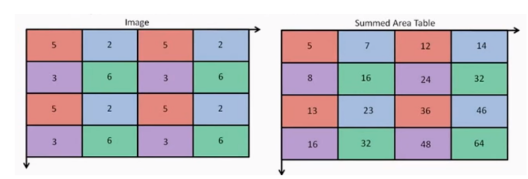
\includegraphics[width=0.7\textwidth]{./pictures/imagenIntegral}
   	\caption{Ejemplo de imagen integral}\label{fig: figura}
   \end{figure}
   El detector de Viola y Jones clasifica las imágenes basado en el valor de simples caracter??sticas, los sistemas basados en caracter??sticas operan muchos más rápido que los basados en píxeles. La imagen integral puede ser usada para estimar el valor de caracter??sticas tipo Haar, las caracter??sticas Haar se visualizan como rectángulos adyacentes blancos y negros, el valor que generan se calcula de la diferencia de la suma de los pixeles en el área blanca menos la suma de los del área negra, la adyacencia que presentan los rectángulos permite reutilizar algunos valores. El conjunto de caracter??sticas rectangulares ofrece una muy buena representación de imágenes la cual soporta un efectivo entrenamiento.
   
   \begin{figure}[htbp]
   	\centering
   	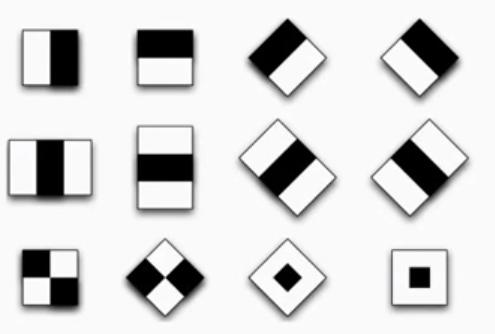
\includegraphics[width=0.4\textwidth]{./pictures/haar}
   	\caption{Características Haar}\label{fig: figura}
   \end{figure}
   
   \subsubsection{Algoritmo AdaBoost}
   Los métodos de Boosting [Friedman et al 2000] básicamente consisten en combinar la eficiencia de muchos clasificadores ?débiles? para producir un poderoso consejo o comité clasificador. El algoritmo Adaboost es el método más usado y práctico de los algoritmos de Boosting. La idea general del AdaBoost consiste en que los ejemplos que son clasificados erróneamente obtienen mayor peso en las iteraciones siguientes, esto significa que los ejemplos que se encuentran cerca de la frontera de decisión son generalmente más dif??ciles de clasificar y por lo tanto se les asigna mayores pesos después de unas cuantas iteraciones. La idea de reasignación de pesos en el conjunto de entrenamiento es esencial en los métodos de Boosting.
   El detector de Viola y Jones se entrenó con conjuntos de imágenes etiquetadas como positivas y negativas, el algoritmo de AdaBoost fue utilizado para entrenar al clasificador y seleccionar un conjunto pequeño con las caracter??sticas Haar más importantes de una muy amplia biblioteca de posibles caracter??sticas. Como resultado final del proceso de entrenamiento el algoritmo de AdaBoost produce un clasificador robusto que tiene la forma de un perceptrón, una combinación de clasificadores débiles en el que cada clasificador tiene asociado una sola caracter??stica Haar y un umbral. Resumiendo lo anteriormente mencionado, la utilización del algoritmo de clasificación AdaBoost permite encontrar las caracter??sticas que mejor separan los ejemplos positivos de los negativos. Una de las ventajas clave por la cual fue elegido AdaBoost como algoritmo seleccionador de caracter??sticas por Viola y jones en su detector, es la increíble velocidad que presenta; usando AdaBoost, un clasificador de 200 caracter??sticas puede ser construido en alrededor 10-11 operaciones de procesador. Las primeras caracter??sticas seleccionadas por AdaBoost tienen mucho sentido y son fáciles de interpretar, una de esas caracter??stica parece enfocarse en la propiedad de que la región de los ojos es por lo regular más oscura que la región de la nariz y las mejillas.
   \begin{figure}[htbp]
   	\centering
   	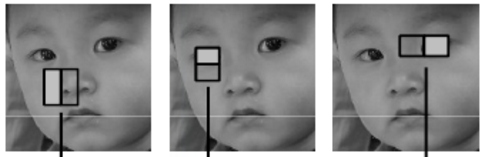
\includegraphics[width=0.7\textwidth]{./pictures/adaboost}
   	\caption{Características tipo Haar sobrepuestas}\label{fig: figura}
   \end{figure}
   
   \subsubsection{Filtro con estructura en cascada.}
   El último componente importante del Detector de Viola y Jones es la estructura en cascada que se forma con la combinación de unos cuantos clasificadores mejorados (boosted), estos clasificadores son usados para rechazar la mayor??a de las subregiones negativas (sin rostros de personas) y poner atención en regiones de la imagen más prometedoras, es decir, las regiones que presenten el rostro de alguna persona. Este método es muy eficiente ya que la mayor??a de las sub-ventanas o subregiones son rechazadas en etapas tempranas. Se le denominó estructura en ?cascada? debido a la forma que presenta al momento de procesar las sub- ventanas. Las sub-ventanas de la entrada del detector pasan a través de una serie de nodos, cada nodo toma una decisión binaria y dependiendo de la decisión la subregión se mueve al siguiente nodo o se rechaza. El número de clasificadores débiles presentes en cada nodo incrementa conforme la sub-ventana se va moviendo a los siguientes nodos, por ejemplo, en el primer nodo contiene un clasificador débil, el segundo 10, el tercero 25, el cuarto 50 y as?? sucesivamente. Teniendo pocos clasificadores en etapas tempranas es otra forma de mejorar la velocidad del detector y esto de alguna forma compensa el costo de evaluar cada caracter??stica Haar en diferentes escalas y posiciones de la imagen.
   \begin{figure}[htbp]
   	\centering
   	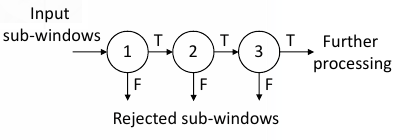
\includegraphics[width=0.7\textwidth]{./pictures/cascada}
   	\caption{Diagrama de nodos}\label{fig: figura}
   \end{figure}
   
   El detector de rostros descrito en esta sección tiene incontables aplicaciones y debido la velocidad de la detección puede ser utilizado en aplicaciones que requieran detección en tiempo real. Uno de los aspectos más interesantes del método de Viola y Jones es que no se limita a la detección de rostros, puede ser modificado para sistemas detectores de otro tipo de patrones en las imágenes, por ejemplo automóviles, peatones y recientemente utilizado para la detección de la enfermedad de Chagas, mediante las muestras de sangre de los infectados [Uc Cetina et al 2015].
   \begin{figure}[htbp]
   	\centering
   	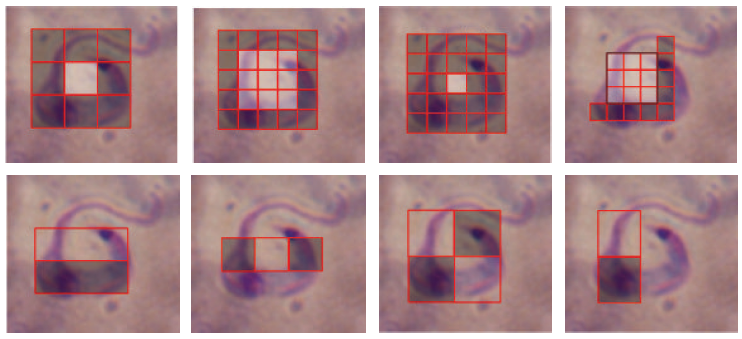
\includegraphics[width=0.7\textwidth]{./pictures/chagas}
   	\caption{Detección de chagas en la sangre mediante el método de Viola y Jones}\label{fig: figura}
   \end{figure}
   

